\documentclass[conference]{IEEEtran}
% CCDC official conference format. Do not override its layout or typography.
\IEEEoverridecommandlockouts
\usepackage{cite}
\usepackage{amsmath,amssymb,amsfonts}
\usepackage{algorithmic}
\usepackage{graphicx}
% Keep floats after their source and within their main section. Subsection
% barriers would force short columns and stretch heading/paragraph spacing.
\usepackage{flafter}
\usepackage[section]{placeins}
\usepackage{textcomp}
\usepackage[table]{xcolor}
\definecolor{methodblue}{HTML}{2376AC}
\usepackage{url}
\def\BibTeX{{\rm B\kern-.05em{\sc i\kern-.025em b}\kern-.08em
    T\kern-.1667em\lower.7ex\hbox{E}\kern-.125emX}}

\title{Engineering Minimum-Cost Reach-Avoid Control for Quadruped Navigation}

\author{
  \IEEEauthorblockN{Anonymous Author(s)}
  \IEEEauthorblockA{\textit{Affiliation}\\
  Address\\
  \texttt{email}}
}

\begin{document}
% Avoid stretching inter-float and heading glue to force equal column bottoms.
\raggedbottom
\maketitle

\begin{abstract}
The deployment of minimum-cost reach-avoid control on a real quadruped robot is investigated. For RC-PPO deployment, the mismatch between its nominal transition model and quadruped locomotion is addressed through a frozen velocity tracker and two data-calibrated margins. Nominal budget accounting is corrected by the cost margin, while the unsafe set is expanded by the geometric margin before high-level learning. Across three navigation scenarios, 73.3\% success and 9.0\% budget violation are attained with the resulting calibrated minimum-cost reach-avoid (CaMRA) system, compared with 70.7\% and 14.0\% for uncalibrated RC-PPO. The distinct roles and deployment limits of these corrections are examined through ablation, held-out calibration, and physical-robot studies. An execution-calibrated engineering pipeline is developed, without extending RC-PPO's deterministic theory to a stochastic safety guarantee.
\end{abstract}

\begin{IEEEkeywords}
quadruped navigation, reach-avoid control, safe robot learning
\end{IEEEkeywords}

\section{Introduction}
Quadruped robots are increasingly used for inspection, exploration, and service
tasks in environments where a navigation policy must do more than reach a target.
The robot must remain collision-free during the whole maneuver while avoiding
unnecessary motion and energy expenditure. These requirements are coupled in
cluttered scenes: a short route may pass close to obstacles, whereas a safer route
may consume more time and actuation. Treating safety and efficiency as independent
reward terms therefore makes the desired trade-off dependent on hand-tuned weights.
Minimum-cost reach-avoid (MCRA) control provides a more direct task description by
requiring goal reachability and trajectory-wide avoidance while minimizing a
cumulative cost~\cite{bansal2017,ganai2024survey}.

Recent work has made MCRA learning practical through RC-PPO~\cite{so2024}.
Within RC-PPO, the state is augmented with a safety indicator and remaining budget,
a reachability value function and budget-conditioned policy are learned, and
the least feasible initial budget is then sought. Safety and cost feasibility in
quadruped navigation are represented jointly through these components.

Deploying this formulation on a physical quadruped requires connecting navigation
decisions to joint-level motion. With direct joint commands, the policy must learn
balance and gait coordination together with collision-free goal reaching. Although
falls, excessive body tilt, and obstacle collisions can be encoded as unsafe
states, these constraints alone do not fully specify coordinated and smooth
locomotion. During early training, unstable motion may prevent the robot from
completing informative navigation rollouts, making route selection and cost
optimization harder to learn. A low-level velocity tracker is therefore pretrained
to address balance, gait coordination, and action smoothness, and is frozen before
high-level learning. Navigation is then learned through a fixed velocity-command
interface using RC-PPO.

Although the low-level controller improves locomotion stability and attenuates
disturbances, residual mismatch remains between the nominal model and actual
execution. The same velocity-command sequence may incur additional cost or produce
path deviations, causing the high-level planner to underestimate budget
consumption or overestimate obstacle clearance. To address these discrepancies,
the low-level controller is frozen, and paired nominal and executed
rollouts are collected with identical initial conditions and command sequences. A
cost margin $\alpha$ and a geometric safety margin $\delta$ are then calibrated from the
empirical distributions of cost overruns and path deviations, respectively. The
running cost used in budget updates is increased by the cost margin to account for
execution-induced overhead, while the unsafe set is expanded by the geometric margin to
accommodate path deviations. High-level policy learning and budget search are
subsequently performed using the calibrated model, and the resulting policy is
deployed through the same frozen controller.

An ideal MCRA learner is connected to a physical closed loop through the proposed
calibrated minimum-cost reach-avoid (CaMRA) deployment pipeline. No strict
stochastic safety guarantee or extension of RC-PPO's deterministic theory to general
stochastic systems is claimed; the scope is limited to empirical robustness under
the execution distribution used to calibrate the margins. The pipeline is evaluated
through controlled mismatch studies, component-wise ablations, sensitivity tests,
and a quantitative physical-robot deployment study. The experiments are designed to
quantify execution mismatch through this fixed interface, assess whether
$\alpha$ and $\delta$ address different failure modes, and evaluate how the
complete system behaves on hardware.

The main contributions are:
\begin{enumerate}
\item An execution-calibrated framework is proposed for quadruped MCRA
      deployment, combining a frozen velocity interface with data-driven cost and
      safety margins to account for model--execution mismatch.
\item A systematic evaluation protocol is developed to assess the distinct
      effects of both margins and characterize system performance and deployment
      limitations through controlled tests and physical-robot evaluation.
\end{enumerate}

\section{Related Work}
\subsection{Minimum-Cost Reach-Avoid Learning}
In reach-avoid reinforcement learning, reaching a target and avoiding an unsafe
set are treated as trajectory-level requirements rather than competing reward terms
\cite{bansal2017,ganai2023}. This formulation is extended to minimum-cost
reach-avoid control in RC-PPO through state augmentation with a safety indicator
and remaining budget, budget-conditioned policy and reachability-critic learning,
and a search for the least feasible initial budget~\cite{so2024}. This construction
is adopted as the algorithmic foundation for connecting nominal MCRA decisions
to quadruped execution.

\subsection{Safe Quadruped Navigation}
A foundation for quadruped navigation in challenging environments is provided by
learning-based locomotion controllers. Robust locomotion on natural terrain
using proprioceptive feedback was demonstrated by Lee et al.~\cite{lee2020},
while rapid motor adaptation was introduced by Kumar et al.~\cite{kumar2021}
to accommodate changes in terrain and payload. At the navigation level, a policy
was trained by Jin et al.~\cite{jin2023resilient} to issue velocity commands to an
existing locomotion controller and respond to perception failures using
locomotion-level observations. In contrast, a joint-level agile policy was
developed by He et al.~\cite{he2024abs}, with reach-avoid-guided switching to a
recovery policy for collision avoidance. A
hierarchical architecture is adopted here, with a frozen velocity tracker handling
locomotion stabilization and a high-level MCRA policy addressing goal reaching,
obstacle avoidance, and cumulative cost.

\subsection{Robust Deployment under Model--Execution Mismatch}
Model uncertainty is addressed through domain randomization and robust
reinforcement learning by broadening the training distribution or optimizing
performance across uncertain dynamics~\cite{tobin2017,smirnova2019,wang2021,liu2022drql}.
In chance-constrained and risk-aware planning, uncertainty is instead incorporated
into planning constraints or risk measures~\cite{theurkauf2023,fan2021step,schmittle2024}. For example, STEP
is used to estimate stochastic traversability for risk-aware off-road
planning~\cite{fan2021step}, while sensing uncertainty is addressed through
multiple long-range planning samples by Schmittle et al.~\cite{schmittle2024}.
Here, residual execution errors under a fixed velocity interface are addressed:
empirical quantiles of paired nominal and executed rollout errors are
used to calibrate cost and geometric margins for MCRA learning and deployment.

\section{Problem Setup: From Ideal MCRA to Quadruped Execution}
\label{sec:problem_setup}
\subsection{MCRA and RC-PPO Recap}
The navigation layer is modeled as a discrete-time process with state $x_t\in
\mathcal{X}$, high-level velocity command $u_t\in\mathcal{U}^{\mathrm{high}}$,
transition kernel $P$, running cost $c$, and initial-state distribution $\rho_0$.
The MCRA objective is to reach a goal set $\mathcal{G}$, avoid an unsafe set
$\mathcal{F}$ at every step, and minimize the accumulated cost until a free terminal
time $T$:
\begin{align}
\min_{\pi,T}\quad &\sum_{t=0}^{T-1}c(x_t,\pi(x_t))\\
\mathrm{s.t.}\quad &x_T\in\mathcal{G},\quad x_t\notin\mathcal{F}\ \forall t\leq T,
\quad x_{t+1}\sim P(\cdot\mid x_t,\pi(x_t)).
\end{align}
The sets are represented using signed functions $g$ and $h$ as
$\mathcal{G}=\{x:g(x)\leq0\}$ and $\mathcal{F}=\{x:h(x)>0\}$. Following
RC-PPO~\cite{so2024}, the state is augmented to $\hat{x}_t=(x_t,y_t,z_t)$,
where $y_t\in\{-1,1\}$ records whether the unsafe set has been entered and $z_t$
is remaining budget. The shifted indicator is
$I_{b\in\mathcal{B}}=+1$ when $b\in\mathcal{B}$ and $-1$ otherwise; thus
$y_{t+1}=\max\{I_{x_{t+1}\in\mathcal{F}},y_t\}$ and
$z_{t+1}=z_t-c(x_t,u_t)$. The augmented goal function is
\begin{equation}
\hat{g}(x,y,z)=\max\{g(x),Cy,-z\},
\end{equation}
where $C>0$ is an arbitrary safety-violation constant. RC-PPO notes that a
practical choice is $C=\max_{x\in\mathcal{X}}g(x)$~\cite{so2024}. Reaching the
zero sublevel set of $\hat{g}$ therefore encodes goal reaching, trajectory-wide
avoidance, and the upper-bound property $z_0\geq\sum_t c_t$. The reachability critic,
budget-conditioned actor, and two-phase minimum-budget search from RC-PPO are
adopted as the high-level decision backbone. Its connection to quadruped closed-loop
execution and the resulting model--execution mismatch are defined below.

\subsection{Quadruped Closed-Loop Execution}
On hardware, $u_t$ is a desired body velocity that is realized by a locomotion
controller. Let $P_{\mathrm{cl}}$ denote the induced closed-loop transition after
this controller is applied. The nominal model used by high-level learning is
$x_{t+1}=\bar f_{\mathrm{cl}}(x_t,u_t)$, while the executed transition is sampled
from $P_{\mathrm{cl}}(\cdot\mid x_t,u_t)$. The difference is the deployment gap
addressed by CaMRA. For a paired nominal/executed rollout, the relative
cost overrun and a trajectory-deviation statistic are defined as
\begin{equation}
\varepsilon_c=\frac{J_{\mathrm{exec}}-J_{\mathrm{nom}}}{J_{\mathrm{nom}}},
\qquad
\varepsilon_d=d(\tau_{\mathrm{exec}},\tau_{\mathrm{nom}}),
\end{equation}
Here $J$ is a nonnegative navigation proxy cost in arbitrary units (a.u.),
not measured electrical energy. Both members of a pair use the same command
program and time window; $d$ is their maximum time-aligned planar position
distance.

\subsection{Deployment Objective and Scope}
The deployment objective is to retain the RC-PPO MCRA semantics while accounting
for the measured distribution of $(\varepsilon_c,\varepsilon_d)$. These quantities
are treated as empirical descriptions of the nominal-to-execution gap rather
than as a new stochastic reachability model. This gap is addressed through a
fixed velocity interface, paired rollout data, and calibrated margins for
high-level learning and deployment.

\section{Execution-Calibrated CaMRA}
% TASK-010--TASK-012: interface, mismatch dataset, alpha/delta calibration,
% robustified RC-PPO learning and deployment algorithm.
\subsection{System Overview}
The CaMRA architecture is shown in Fig.~\ref{fig:system_overview}. A high-level
MCRA navigation policy is coupled with a pretrained, frozen low-level velocity
tracker. The system is developed in two stages. First, the tracker is trained and
frozen, and paired nominal and executed rollouts are collected to calibrate the
cost margin $\alpha$ and geometric margin $\delta$. Second, these margins are
incorporated into RC-PPO-based high-level learning and initial-budget selection.
During deployment, body-velocity commands are generated by the navigation policy
and converted into joint commands by the frozen tracker for closed-loop execution.

\begin{figure}[!htbp]
\centering
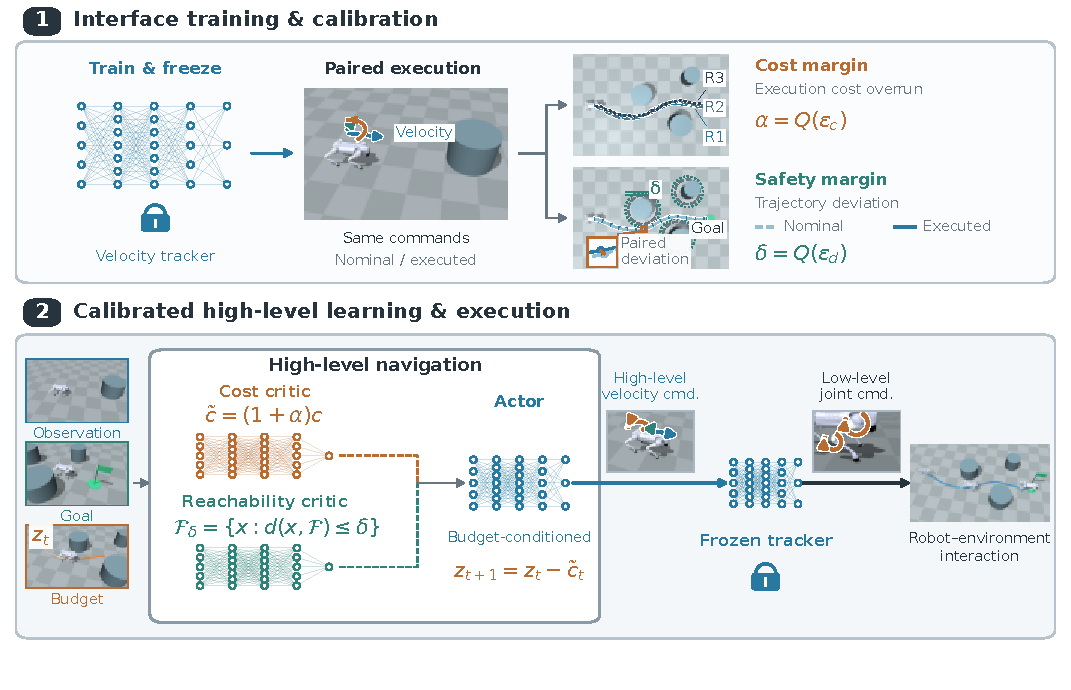
\includegraphics[width=\columnwidth]{../../images/1020/deployment_calibration_overview.pdf}
\caption{CaMRA architecture. In Stage 1, a frozen velocity interface is established
and execution margins are calibrated. In Stage 2, the margins are incorporated into
high-level navigation learning and budget selection, with the same tracker retained for execution.
Scenes and paths are schematic; successive robot states are represented by ghost poses.}
\label{fig:system_overview}
\end{figure}

\subsection{Hierarchical Control with a Frozen Velocity Interface}
Direct joint-level MCRA learning would require a quadruped policy to acquire stable
locomotion while learning goal reaching, obstacle avoidance, and cost reduction.
Although falls and excessive body tilt can be represented as unsafe states,
avoiding these states alone provides limited guidance for learning coordinated and
smooth locomotion. Frequent loss of balance during early training can also
interrupt navigation exploration. A hierarchical architecture is therefore adopted
to separate locomotion stabilization from high-level reach-avoid decisions.

The low-level tracker is pretrained using PPO and domain randomization to track
velocity commands while maintaining balance, gait coordination, and action
smoothness. Proprioceptive observations and body-velocity commands
$u_t=[v_x^*,v_y^*,\omega_z^*]^\top$ are mapped to joint commands. Execution
disturbances are attenuated through closed-loop feedback within the trained command domain. The tracker is
then frozen before mismatch calibration and high-level learning, preventing
subsequent low-level parameter updates from changing the execution interface. The
high-level policy is consequently trained through velocity commands rather than
directly on joint coordination.

The nominal map $\bar f_{\mathrm{cl}}$ abstracts this interface by integrating
commanded body velocities over each high-level decision interval under ideal
tracking. Contact variation, friction, actuation latency, and state-estimation
errors can nevertheless cause deviations from this abstraction. The same frozen
tracker and command domain are retained for calibration, high-level learning, and
deployment, providing a consistent basis for measuring residual mismatch and
calibrating the margins in the next subsection.

\subsection{Execution-Mismatch Calibration}
\label{sec:execution_calibration}
To convert execution mismatch into cost and safety margins, paired nominal and
executed rollouts are collected through the frozen velocity interface. For each
pair, the same initial state, map, goal, and high-level command sequence are used
in the nominal model and a perturbed execution. For a rollout of length $T$,
let
$J_{\rm nom}=\sum_{t=0}^{T-1}c(x_t^{\rm nom},u_t)$ and
$J_{\rm exec}=\sum_{t=0}^{T-1}c(x_t^{\rm exec},u_t)$. Disjoint rollouts are used
for calibration and independent evaluation; evaluation data are excluded from margin selection.

For $J_{\rm nom}>0$, the relative cost overrun $\varepsilon_c$ is computed from
the paired cumulative costs using the definition in Section~\ref{sec:problem_setup}. For geometric
deviation, the maximum planar distance between time-aligned base positions is used,
\begin{equation}
\varepsilon_d=\max_{0\leq t\leq T} \left\|p_t^{\rm exec}-p_t^{\rm nom}\right\|_2,
\end{equation}
where $p_t$ is the base position.

The two errors are calibrated separately because they affect different MCRA
constraints. For quantile levels $p_c$ and $p_d$, the margins are set to
\begin{equation}
\alpha=Q_{p_c}(\varepsilon_c),\qquad
\delta=Q_{p_d}(\varepsilon_d),
\end{equation}
where $Q_p$ denotes the empirical $p$-quantile of the calibration samples. The
calibrated running cost is
$\tilde c(x_t,u_t)=(1+\alpha)c(x_t,u_t)$, so the remaining budget evolves as
$z_{t+1}=z_t-\tilde c(x_t,u_t)$. The unsafe set is dilated to
$\mathcal{F}_\delta=\{x:d(x,\mathcal{F})\leq\delta\}$. Both margins are determined
before high-level learning and are held fixed, with empirical coverage tied to the
execution conditions represented in the calibration data.

\subsection{Robust MCRA Learning and Deployment}
A budget-conditioned navigation policy is trained using the calibrated cost and
expanded unsafe set, and an initial budget is selected for execution through the
frozen velocity interface. The margins are incorporated into learning, so navigation
decisions are optimized under the corrected cost and safety conditions.

In Phase I, budget updates are computed using the calibrated running cost $\tilde c$,
while the safety indicator and augmented goal are determined from the expanded
unsafe set $\mathcal{F}_\delta$. A stochastic actor
$\pi_\theta(u\mid o,y,z)$ and two critics are employed: goal reaching and safety
are evaluated by $V_h$, and corrected cumulative cost is estimated by $V_c$ over
the same stopping horizon. With
cost normalized by $z_{\rm ref}$, the combined residual is
\[
W=\max\{V_h,V_c-z/z_{\rm ref}\}.
\]
The actor is optimized to reduce this residual. Accordingly, cost targets and
budget updates are modified through $\alpha$, whereas reachability targets are
modified through $\delta$ via the safety indicator.

In Phase II, a deterministic deployment policy is obtained from the actor's mean
action, and the critics are refitted with the actor fixed. Candidate initial
budgets are evaluated under the calibrated model, and the smallest tested budget
satisfying the prescribed goal-reaching, collision, and budget-violation criteria
is selected.

During deployment, navigation observations and the remaining budget are supplied
to the policy. The resulting body-velocity commands are executed through the
frozen tracker. The calibrated cost used to update the remaining budget is
obtained from a parallel nominal rollout driven by the same commands.

\section{Experiments}
% Evaluation: overall performance, calibration mechanisms, budget sensitivity,
% execution perturbations, and hardware deployment.
\subsection{Experimental Setup and Evaluation Protocol}
\label{sec:experimental_setup}
Navigation performance, execution-error calibration, margin contributions and
sensitivity, budget selection, robustness to execution disturbances, and physical
deployment are evaluated. High-level decisions through the velocity interface are
assessed in the planar navigation benchmark, while quadruped execution is examined
in the hardware study.

The navigation benchmark comprises moderately cluttered, narrow-passage, and
densely obstructed maps, each spanning $8\times8$ m. Test maps, navigation
observations, command limits, and the frozen velocity tracker are shared across
methods, with matched training interaction budgets and network widths. The high-level decision
interval is 0.2 s, and the episode horizon is 30 s. Each method is evaluated using
three trained policies from different random seeds, with 100 trials per policy
and scenario, yielding 300 trials per scenario and 900 overall. Separate rollout
sets are used for calibration, training, budget selection, and final evaluation.

Five metrics are reported: success rate (SR), mean executed cost (Cost), physical
collision rate (CR), budget violation rate (BVR), and mean per-trial minimum
clearance (MC). Success requires collision-free goal reaching before timeout;
budget compliance is assessed separately. Collision and clearance are measured
against a common physical robot footprint. All trials until goal reaching,
collision, or timeout are included in Cost and MC; evaluation is continued after
budget exceedance. Equally weighted scenario means are reported in the tables at $z_0/z_{\rm ref}=1$,
with reference budgets of 120, 140, and 190 a.u. Scenario-level intervals describe
test-case variability conditional on the trained policies.

The baselines comprise uncalibrated RC-PPO, reach-avoid learning without cost
conditioning (RA), reward-based PPO, and constrained PPO (CPPO). For RC-PPO,
$\alpha=\delta=0$ is used, while the budget input is omitted for RA. PPO and CPPO are evaluated
with low and high safety weights, $\beta_L=1$ and $\beta_H=5$; CPPO additionally
is subject to an expected-cost constraint.

\subsection{Overall Navigation Performance}
\label{sec:overall_performance}
The complete pipeline is compared with the baselines in Table~\ref{tab:main_results},
and the same five metrics are reported by scenario in Fig.~\ref{fig:metrics_draft}.
Compared with uncalibrated RC-PPO, mean SR is increased from 70.7\% to
73.3\%, mean executed cost is reduced from 91.7 to 88.3 a.u., and BVR is lowered from
14.0\% to 9.0\% with CaMRA, with similar CR (15.7\% versus 15.0\%). Lower CR
and greater clearance are obtained with RA and CPPO$_{\beta_L}$, but with lower
SR and higher cost and BVR. A joint success--safety--cost trade-off is thus observed.

\begin{table}[!htbp]
\caption{Equal-scene mean performance at $z_0/z_{\rm ref}=1$.
Cost is interpreted jointly with SR.}
\label{tab:main_results}
\centering
\small
\setlength{\tabcolsep}{3pt}
\renewcommand{\arraystretch}{1.12}
\begin{tabular}{@{}lccccc@{}}
\hline
Method & \shortstack{SR\\(\%) $\uparrow$} & Cost & \shortstack{CR\\(\%) $\downarrow$} & \shortstack{BVR\\(\%) $\downarrow$} & \shortstack{MC\\(m) $\uparrow$}\\
\hline
\rowcolor{methodblue!9}
\textbf{CaMRA} & \textbf{73.3} & \textbf{88.3} & 15.0 & \textbf{9.0} & 0.31\\
RC-PPO & 70.7 & 91.7 & 15.7 & 14.0 & 0.30\\
RA & 60.0 & 104.0 & 13.0 & 20.0 & 0.34\\
PPO$_{\beta_L}$ & 67.7 & 99.7 & 23.0 & 20.7 & 0.20\\
PPO$_{\beta_H}$ & 42.3 & 117.0 & 29.0 & 27.0 & 0.16\\
CPPO$_{\beta_L}$ & 37.7 & 124.7 & \textbf{12.3} & 22.3 & \textbf{0.36}\\
CPPO$_{\beta_H}$ & 69.7 & 105.7 & 18.3 & 17.0 & 0.26\\
\hline
\end{tabular}
\end{table}

\begin{figure}[!htbp]
\centering
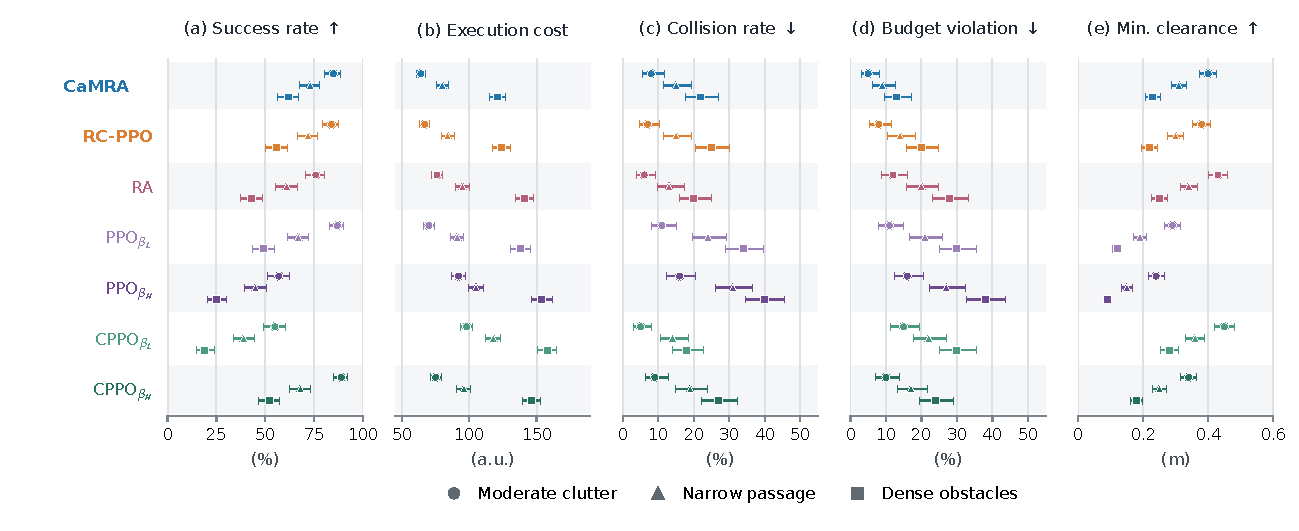
\includegraphics[width=\columnwidth]{../../images/1020/metrics_comparison.pdf}
\caption{Scenario-level SR, Cost, CR, BVR, and MC at the common reference budget.
Scenarios and methods are distinguished by markers and colors, respectively.
Estimates and 95\% intervals conditional on the three trained policies are shown
as points and horizontal bars ($n=300$ per method and scene). Equal-scene means
are reported in Table~\ref{tab:main_results}.}
\label{fig:metrics_draft}
\end{figure}

Navigation behavior in one paired example is illustrated in
Fig.~\ref{fig:trajectory_sync}. With the geometric margin $\delta$, a slightly
longer, more costly route with greater obstacle clearance is followed with CaMRA.
Obstacle passages are related to clearance, executed cost, and tracking error in
the synchronized curves, while the role of $\alpha$ in budget accounting is shown
by the corrected nominal charge. The common budget is satisfied by both methods,
illustrating a safety--cost trade-off. The same proxy cost definition is used in
this separate diagnostic case, which is excluded from Table~\ref{tab:main_results}.

\begin{figure}[!htbp]
\centering
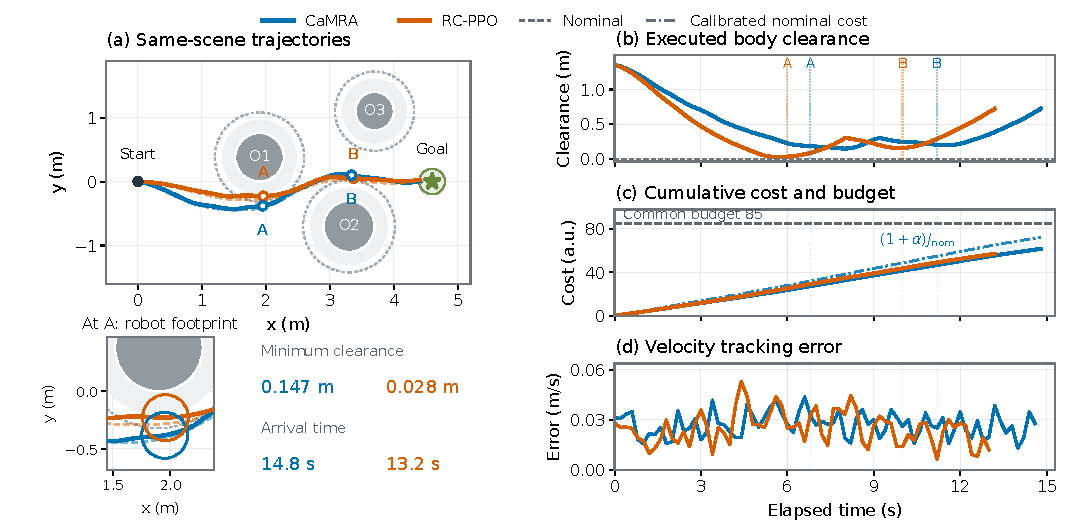
\includegraphics[width=\columnwidth]{../../images/1020/trajectory_sync.pdf}
\caption{Same-scene trajectories and synchronized diagnostics for CaMRA (blue)
and RC-PPO (orange), with a common initial budget of 85 a.u.
(a) Executed (solid) and nominal (dashed) paths, with $\delta=0.12$ m.
(b) Physical clearance. (c) Cumulative costs, budget, and corrected charge
$(1+\alpha)J_{\rm nom}$, with $\alpha=0.18$. (d) Linear-velocity tracking error.
Each method's obstacle passages are marked by A/B; traces are truncated at the
respective terminations.}
\label{fig:trajectory_sync}
\end{figure}

\FloatBarrier
\subsection{Execution-Error Calibration and Margin Analysis}
\label{sec:mismatch_analysis}
Execution mismatch is summarized in Fig.~\ref{fig:margin_calibration} using 800
calibration and 400 held-out paired rollouts. The
calibration medians are $0.09$ for relative cost overrun and $0.06$ m for maximum
planar position deviation; $\alpha=0.18$ and $\delta=0.12$ m are selected from
their 90th percentiles. With these margins fixed, held-out coverage is $353/400$
($88.25\%$) for cost and $346/400$ ($86.50\%$) for position. These marginal
coverages are used to assess the error allowances in budget accounting and obstacle
inflation; joint held-out coverage is $336/400$ ($84.0\%$). Neither marginal nor
joint error coverage is a navigation success probability.

\begin{figure}[!htbp]
\centering
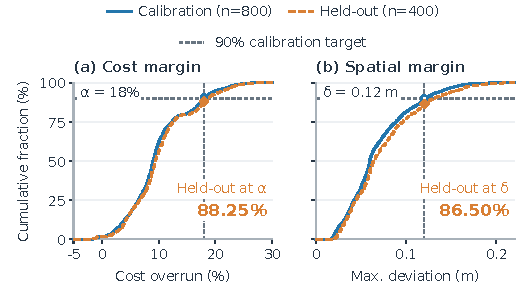
\includegraphics[width=\columnwidth]{../../images/1020/margin_calibration.pdf}
\caption{Execution-error calibration and held-out assessment.
Calibration and held-out empirical CDFs are shown as blue solid and orange dashed
curves. The calibration 90th percentiles and 90\% target are marked by vertical
and horizontal lines, respectively. Coverage at the fixed thresholds, including
ties, is indicated by circles and diamonds.}
\label{fig:margin_calibration}
\end{figure}

The effects of the cost and safety corrections are isolated in
Table~\ref{tab:ablation_draft} by removing $\alpha$, $\delta$, or both while
retaining the same frozen velocity tracker. These comparisons are visualized in
Fig.~\ref{fig:ablation_margins}. Without $\alpha$, BVR is increased by
13.4 percentage points; without $\delta$, CR is increased by 11.3 percentage
points and clearance is reduced.

\begin{table}[!htbp]
\caption{Margin ablation with the same frozen tracker and reference budget as
Table~\ref{tab:main_results}.
Cost is interpreted jointly with SR.}
\label{tab:ablation_draft}
\centering
\small
\setlength{\tabcolsep}{3pt}
\renewcommand{\arraystretch}{1.12}
\begin{tabular}{@{}lccccc@{}}
\hline
Variant & \shortstack{SR\\(\%) $\uparrow$} & Cost & \shortstack{CR\\(\%) $\downarrow$} & \shortstack{BVR\\(\%) $\downarrow$} & \shortstack{MC\\(m) $\uparrow$}\\
\hline
\rowcolor{methodblue!9}
\textbf{CaMRA} & \textbf{73.3} & 88.3 & \textbf{15.0} & \textbf{9.0} & \textbf{0.31}\\
w/o both (RC-PPO) & 70.7 & 91.7 & 15.7 & 14.0 & 0.30\\
w/o $\alpha$ & 67.2 & 80.6 & 19.8 & 22.4 & 0.29\\
w/o $\delta$ & 64.8 & \textbf{77.2} & 26.3 & 13.8 & 0.19\\
\hline
\end{tabular}
\end{table}

The CaMRA and RC-PPO results from Table~\ref{tab:main_results} are reused for
the full and zero-margin rows. Each single-margin variant is trained separately:
the effects are non-additive, and lower cost can accompany more failed or
shorter trials. Cost must therefore be interpreted jointly with success rate.

\begin{figure}[!htbp]
\centering
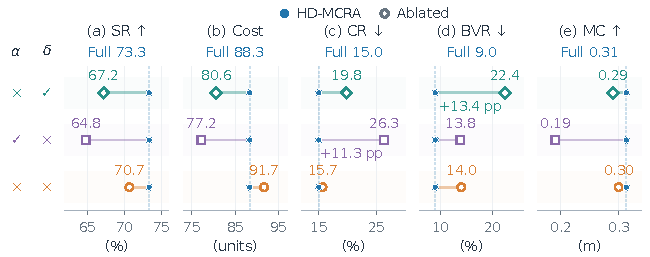
\includegraphics[width=\columnwidth]{../../images/1020/ablation_horizontal.pdf}
\caption{Effects of removing the cost margin $\alpha$ and geometric margin
$\delta$ at the common reference budget. Changes between variants are indicated
by connecting lines.}
\label{fig:ablation_margins}
\end{figure}

To assess margin sensitivity beyond component removal, the high-level networks
are retrained for each of 16 combinations
of $\alpha\in\{0,0.09,0.18,0.27\}$ and
$\delta\in\{0,0.06,0.12,0.18\}$ m, retaining the frozen tracker, training
budget, and 900-trial evaluation protocol. The four zero/calibrated combinations
match Table~\ref{tab:ablation_draft}. With both margins increased to $(0.27,0.18)$,
CR and BVR are reduced to 13.3\% and 6.7\%, but SR is lowered to 68.0\% and
cost is raised to 95.0 a.u. A conservatism trade-off is thus observed with larger margins.
Calibration is performed before the sweep and is not retuned to maximize these
results.

\FloatBarrier
\subsection{Budget Selection and Performance Trade-offs}
\label{sec:budget_sensitivity}
With policy parameters and margins fixed, the effect of initial budget on
navigation performance is evaluated. Budget selection is performed on a separate
rollout set, while Fig.~\ref{fig:budget_draft} reports performance on the final
evaluation set. Since RA is not conditioned on budget, the same trajectories are
evaluated at each threshold, and only its BVR changes. Under the criteria
SR $\geq60\%$, CR $\leq20\%$, and BVR $\leq15\%$, the smallest tested budget
ratios satisfying all three criteria on the final response curves are $0.90$
for CaMRA, $0.96$ for RC-PPO, and $1.12$ for RA. The same evaluation criteria
are therefore met at a lower tested budget with CaMRA.
\begin{figure}[!htbp]
\centering
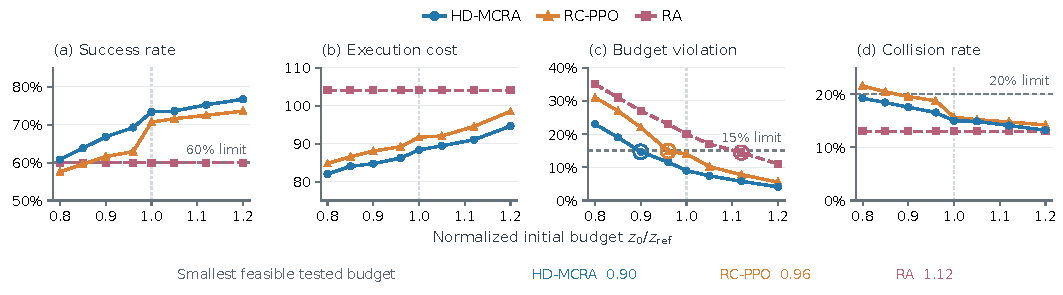
\includegraphics[width=\columnwidth]{../../images/1020/budget_sweep_horizontal.pdf}
\caption{Budget-response curves averaged equally across scenarios. Acceptance
thresholds are indicated by dashed lines; the smallest tested budgets satisfying
all three criteria are marked by outlined points. Results at the reference budget match
Table~\ref{tab:main_results}.}
\label{fig:budget_draft}
\end{figure}

\FloatBarrier
\subsection{Robustness to Execution Perturbations}
\label{sec:execution_robustness}
With the policy and margins fixed, performance is evaluated as
execution conditions depart from calibration. Each profile's deviation from
the nominal condition is increased by 25\%: the lowest friction becomes
0.4875, maximum delay becomes 0.125 s, and maximum
velocity-noise standard deviation becomes 0.05 m/s. Across 900 independent
trials (60 per profile and scene), SR is
$65.0\%$ and BVR $16.0\%$ for CaMRA versus SR $58.0\%$ and BVR $24.0\%$ for
uncalibrated RC-PPO. Their respective CR values are 22.0\% and 27.0\%, costs
are 96.8 and 102.4 a.u., and MC values are 0.26 and 0.24 m. No policy or margin
is refitted for this stress test. Under the tested perturbations, higher success
and lower collision and budget-violation rates are obtained with CaMRA than with
uncalibrated RC-PPO.

\subsection{Physical-Robot Deployment and Failure Analysis}
\label{sec:hardware_deployment}
A Unitree Go2 is used in two cluttered indoor settings. An obstacle-filled
corridor is shown in Fig.~\ref{fig:hardware_sequences}(a), where collision
avoidance during traversal is examined. A chair arrangement with multiple
available routes is shown in Fig.~\ref{fig:hardware_sequences}(b), where low-cost
route selection under obstacle constraints is examined.

\begin{figure}[!htbp]
\centering
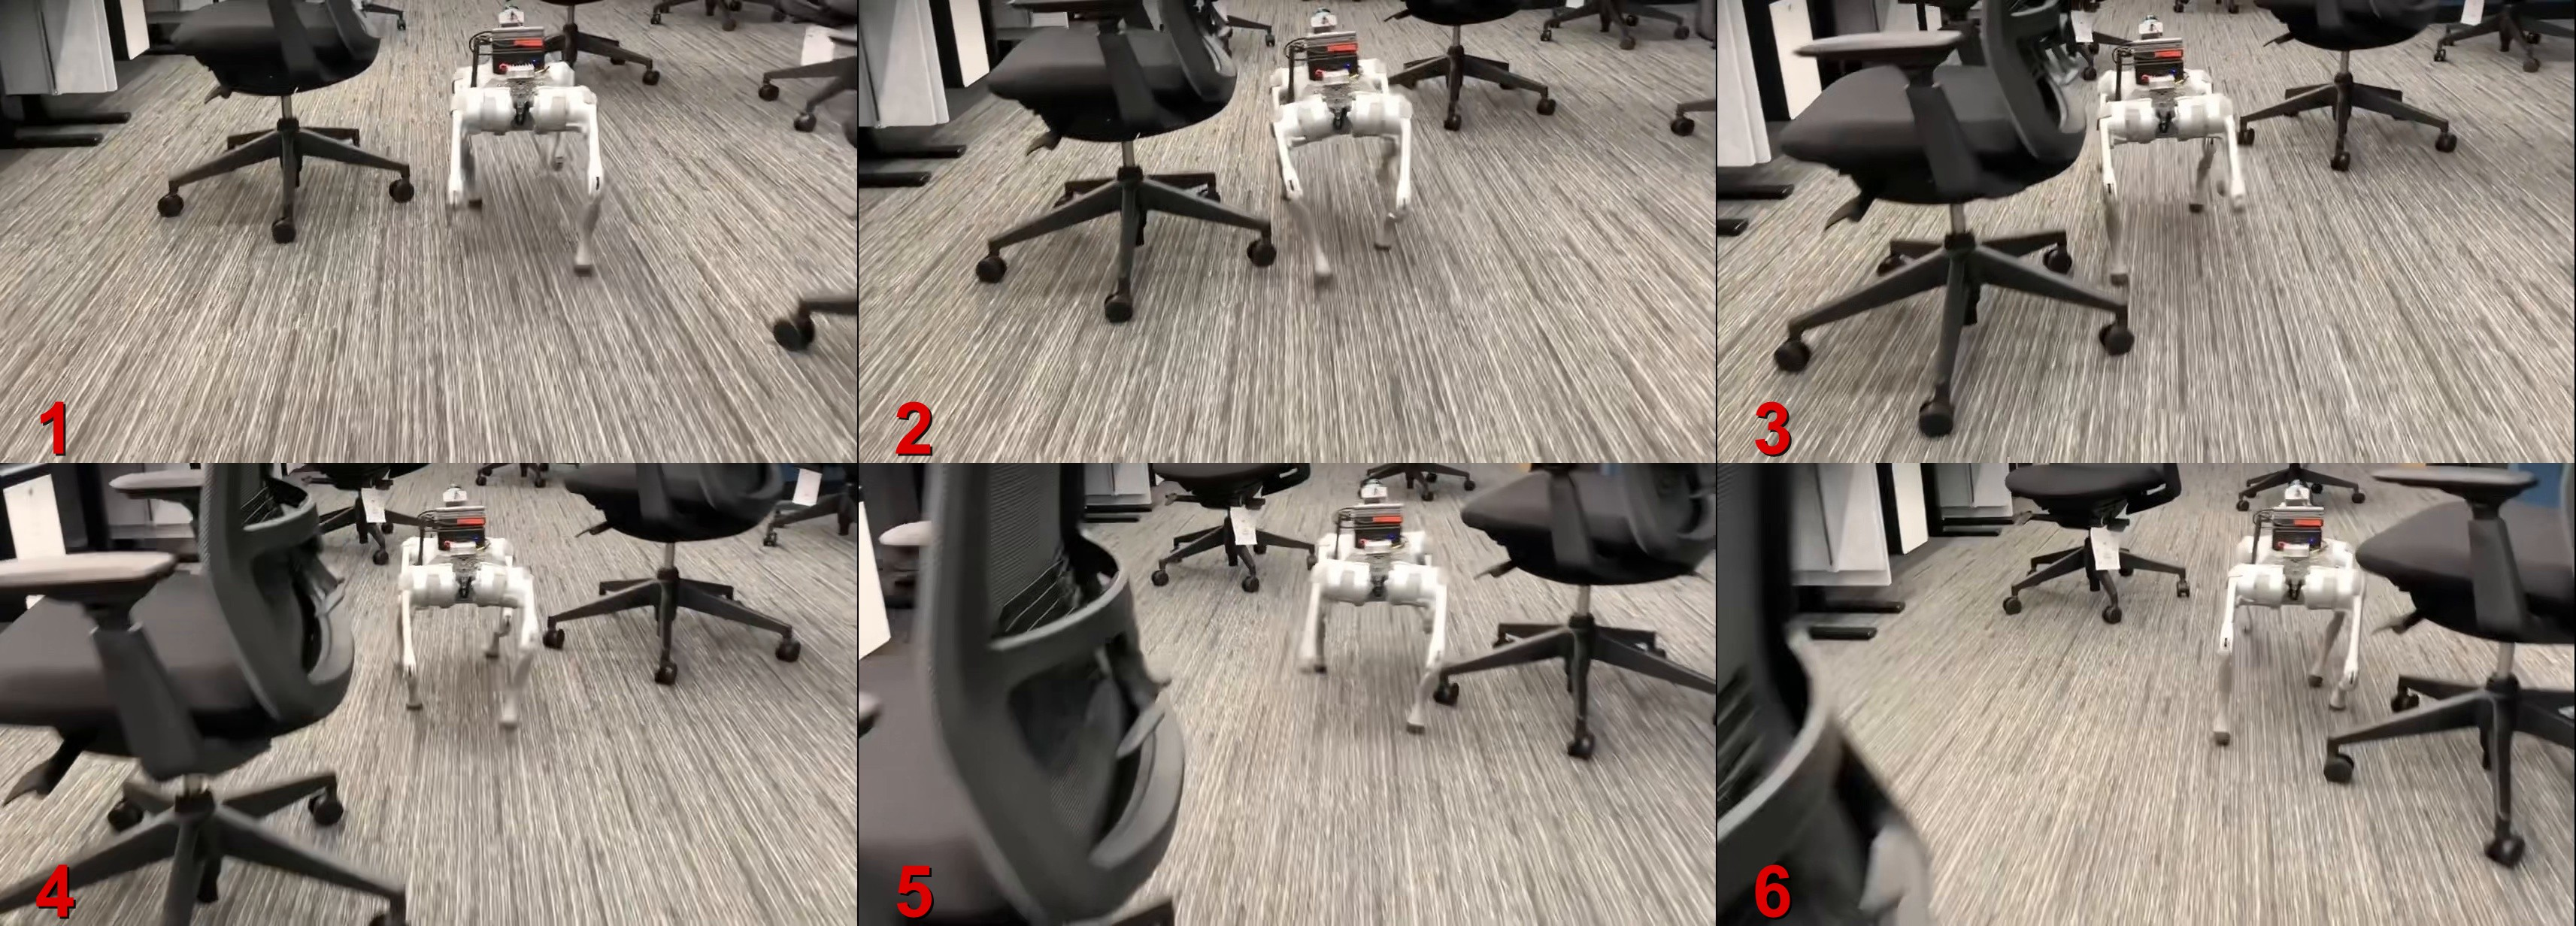
\includegraphics[width=\columnwidth]{../../images/1020/office_sequence_candidate_A_numbered.jpg}
\par\smallskip
{\footnotesize (a) Obstacle avoidance in a cluttered corridor.\par}
\medskip
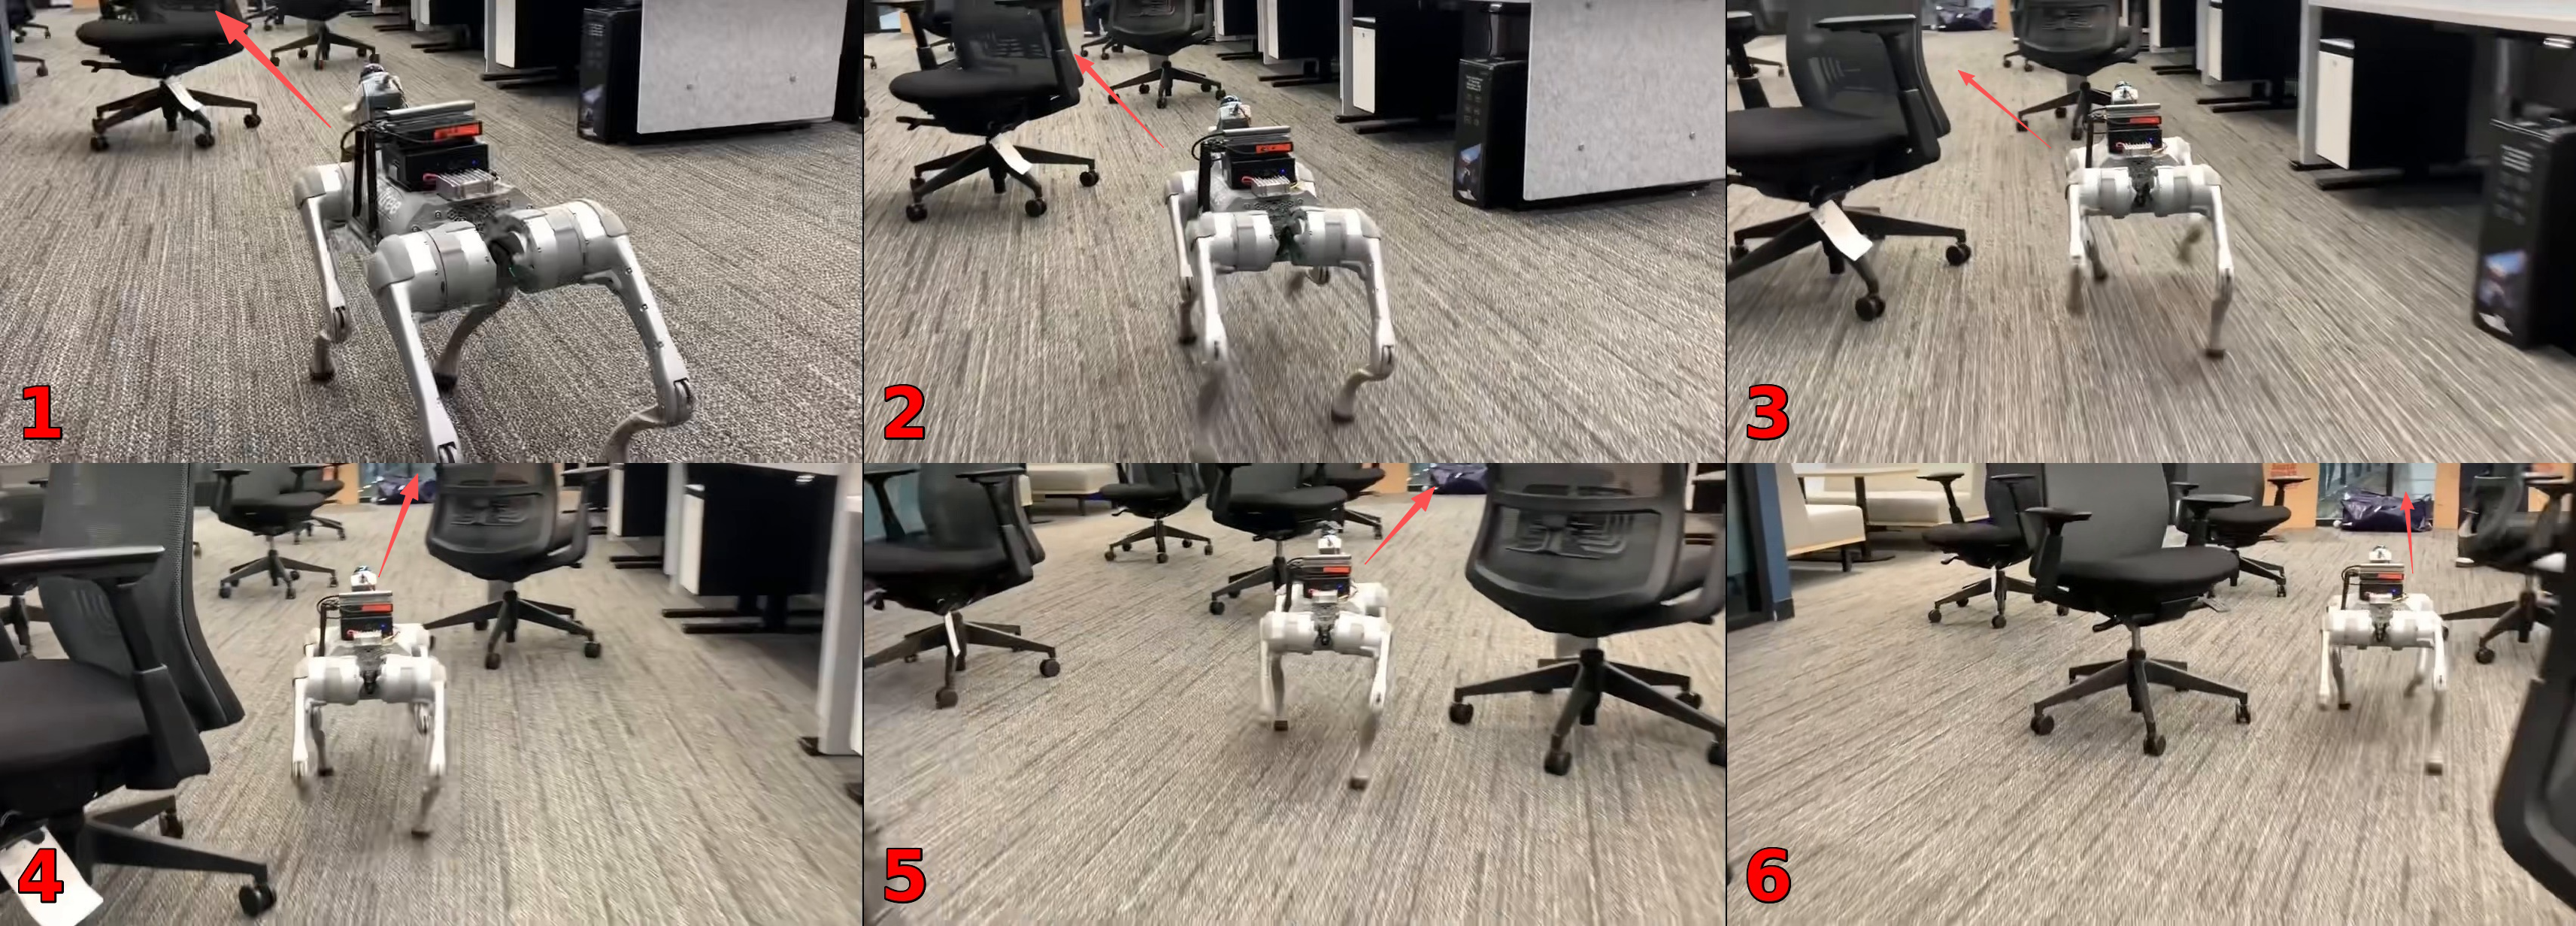
\includegraphics[width=\columnwidth]{../../images/1020/office_shortest_path_sequence_final.png}
\par\smallskip
{\footnotesize (b) Low-cost route selection among chair obstacles.\par}
\caption{Physical deployment of Unitree Go2: (a) corridor traversal with obstacle
avoidance; (b) route selection among multiple passages formed by chairs. Each
panel is composed of six successive frames in temporal order; the travel direction
is indicated by red arrows in (b).}
\label{fig:hardware_sequences}
\end{figure}

The representative route is
approximately 15 m, with a narrow passage about 0.3 m wider than the robot
body. Proprioception is provided by joint encoders and the IMU; navigation
observations are obtained from projected LiDAR ranges and local scan matching.
Policies are executed on an onboard x86-64 CPU with 16 GB RAM, at the same
50 Hz/5 Hz control rates. A 60 s horizon and budget 230 a.u. are used for the
15 m task; the tracker, navigation policy, and margins are held fixed.

CaMRA is compared with uncalibrated RC-PPO in Table~\ref{tab:hardware_comparison}
under matched scene conditions, starts, goals, and budget. The same frozen tracker
and navigation inputs are used for both methods; their high-level policies are fixed
throughout evaluation.

\begin{table}[!htbp]
\caption{Synthetic hardware-comparison example, with 50 trials per method.
Cost is in a.u. and is interpreted jointly with SR.}
\label{tab:hardware_comparison}
\centering
\small
\setlength{\tabcolsep}{3pt}
\renewcommand{\arraystretch}{1.12}
\begin{tabular}{@{}lccccc@{}}
\hline
Method & \shortstack{SR\\(\%) $\uparrow$} & Cost & \shortstack{CR\\(\%) $\downarrow$} & \shortstack{BVR\\(\%) $\downarrow$} & \shortstack{MC\\(m) $\uparrow$}\\
\hline
\rowcolor{methodblue!9}
\textbf{CaMRA} & \textbf{70.0} & 182.0 & \textbf{16.0} & \textbf{14.0} & \textbf{0.09}\\
RC-PPO & 64.0 & \textbf{176.0} & 20.0 & 22.0 & 0.07\\
\hline
\end{tabular}
\end{table}

Success counts are $35/50$ for CaMRA and $32/50$ for RC-PPO. Both methods
have three localization aborts; the other failures comprise four timeouts and eight contacts
for CaMRA, versus five timeouts and ten contacts for RC-PPO. BVR decreases
from 22.0\% to 14.0\%, while mean cost increases from 176.0 to 182.0 a.u.
These example values illustrate a clearance--cost trade-off: shorter routes and
earlier failures can lower mean cost without reducing its upper tail.
Every terminal outcome is included in Cost and MC; results are reported separately
from the planar benchmark because of the different route, horizon, and footprint.

\FloatBarrier

\section{Limitations}
Calibration quantiles do not guarantee
coverage under temporal correlation, rare contacts, or distribution shift.
A fixed $\alpha$ can be excessive in open space yet insufficient under actuator
or perception faults; a fixed $\delta$ can eliminate feasible narrow passages.
LiDAR can miss thin or occluded structures. The small indoor hardware study also
requires extension across terrain, payload, and weather conditions. The planar
benchmark simplifies whole-body geometry, and the reported intervals condition
on a small fixed policy bank rather than quantifying new-training-seed variation.

\section{Conclusion}
The inherited RC-PPO objective and solver are connected to a quadruped through
a frozen velocity interface and paired execution calibration in CaMRA. Separate
corrections $\alpha$ and $\delta$ are determined from cost overrun and path
deviation. Empirical robustness within the calibration distribution is addressed
by this engineering layer, without a new stochastic reach-avoid guarantee. The
need to address cost accounting and geometric clearance separately is supported
by the comparisons and ablations. Their benefits must be assessed jointly with goal-reaching: larger
margins can reduce violations while excluding useful routes.

\bibliographystyle{IEEEtran}
\bibliography{references}

% Start the appendices on a new page after the complete reference list.
\clearpage
\appendices
\section{Velocity-Interface Implementation Details}
\label{app:velocity_interface}
The tracker is supplied with 48 inputs: body linear and angular velocities, projected
gravity, the three velocity commands, 12 joint-position offsets, 12 joint
velocities, and 12 previous actions. ELU multilayer perceptrons with widths
512--256--128 are used for the actor and critic. Twelve clipped actions are used to specify
$q^{\rm des}=q^{\rm stand}+0.25a$ rad, subject to joint limits.
The command domain is $v_x^*\in[-0.6,0.6]$ m/s,
$v_y^*\in[-0.4,0.4]$ m/s, and $\omega_z^*\in[-1.2,1.2]$ rad/s.
The tracker and position PD loop are executed at 50 Hz and 200 Hz, respectively, with gains
$K_p=20$ Nm/rad and $K_d=0.5$ Nm\,s/rad. A high-level command is held for
ten tracker updates.

PPO pretraining is performed with 4,096 parallel environments, 24-step rollouts, 1,000
updates, five epochs, four minibatches, Adam learning rate $10^{-3}$,
discount 0.99, GAE parameter 0.95, clip 0.2, entropy coefficient 0.01,
and gradient-norm limit 1. The tracking rewards are
$\exp(-\|v_{xy}-u_{xy}\|^2/0.25)$ and
$0.5\exp(-(\omega_z-u_z)^2/0.25)$. Penalties are
$2v_z^2$, $0.05\|\omega_{xy}\|^2$, squared horizontal projected gravity,
$2{\times}10^{-5}\|\tau\|^2$, and $0.01\|a_t-a_{t-1}\|^2$.
Coordination is encouraged by a first-contact reward of $0.5(t_{\rm air}-0.25)$
per foot when $\|u_{xy}\|>0.1$ m/s. Episodes are terminated after 20 s or upon
body height below 0.18 m or roll/pitch magnitude above 0.8 rad.

During training, friction is randomized over $[0.5,1.25]$, mass and motor-strength
multipliers over $[0.9,1.1]$, and command delay over 0--40 ms. Observation
noise standard deviations are 0.02 m/s and 0.03 rad/s; planar velocity
perturbations up to 0.25 m/s are applied every 8 s. Network parameters and
observation-normalization statistics are frozen together before calibration.
These settings are used for locomotion training; deployment error is not bounded by them.

\section{Execution-Mismatch Calibration Details}
\label{app:calibration_details}
\subsection{Paired-Rollout Configuration}
The 1,200 pairs comprise four command families crossed with five execution
conditions. Straight motion with speed changes, broad arcs, alternating bends,
and stop--turn maneuvers last 12, 16, 20, and 14 s, respectively.
For straight motion, $v_x=0.15$--$0.6$ m/s and small lateral/yaw commands are used;
for arcs, $v_x=0.2$--$0.5$ m/s and yaw magnitudes 0.2--0.8 rad/s are used;
for alternating bends, $v_x=0.15$--$0.5$ m/s and opposite yaw commands of
0.4--1.0 rad/s are used. In stop--turn programs, $v_x=0$--$0.4$ m/s is alternated
with yaw commands of 0.3--1.0 rad/s. Commands are changed at 1 s intervals with
0.2 s ramps and are constrained to the tracker domain.

Friction 0.8, zero added delay, and zero added velocity noise are used for
nominal conditions. Execution conditions $(\mu,d,\sigma_v)$ are
$(0.8,0.02,0.01)$, $(0.55,0.02,0.015)$,
$(0.8,0.10,0.01)$, $(0.8,0.02,0.04)$, and
$(0.55,0.10,0.04)$, with delay in seconds and noise in m/s.
The delay range in pretraining is deliberately exceeded by the 100 ms conditions.
From each of the 20 cells, 40 calibration and 20 independently held-out pairs
are obtained. The same commands are replayed from the same initial state in both
members; only pairs completed over the prescribed common window in a contact-free
calibration arena are accepted. Incomplete or invalid records are excluded before splitting,
without filtering on error magnitude. LiDAR noise is excluded from margin
fitting; 0.02 m range noise and 5\% dropped rays are used for observation-error
checks, with dropped rays filled at maximum range.

For the execution-perturbation study, each profile's deviation from the nominal
condition is scaled by 1.25. The perturbed friction is
$\mu'=0.8+1.25(\mu-0.8)$, giving a minimum of
$0.8-1.25(0.8-0.55)=0.4875$; delay and velocity-noise standard deviation are
scaled as $d'=1.25d$ and $\sigma_v'=1.25\sigma_v$, giving maxima of
0.125 s and 0.05 m/s. Each profile is evaluated in 60 independent trials per
scenario, yielding 900 trials per method across the five profiles and three
scenarios. Policies and margins remain fixed.

\subsection{Measurement and Geometry Conventions}
For interval length $\Delta t=0.2$ s, the running proxy cost is
\begin{equation}
\begin{split}
c_t=\Delta t\big[&3.6+3\|v_{xy,t}\|^2+
20\|v_{xy,t}-u_{xy,t}\|^2\\
&+2\max(0,0.45-\ell_t)\big],
\end{split}
\end{equation}
where $\ell_t$ is physical footprint clearance in metres. Velocities are in
m/s; coefficients define a.u., not joules. Costs are computed using interval-start
clearance and interval-average velocity, and accumulated through goal, contact, or timeout.
The positive time term makes $J_{\rm nom}>0$ for every nonempty pair;
zero-duration records are invalid. Nominal velocity is the commanded velocity
in the planar abstraction; executed velocity is measured separately.
This same cost definition is used for the diagnostic case and navigation benchmarks.

Positions are linearly interpolated onto the common command clock; the maximum
Euclidean discrepancy is measured over the full prescribed window, without phase alignment.
A disc of radius 0.20 m is used for the planar benchmark, while a yaw-oriented
$0.70\times0.32$ m footprint including the leg envelope is used for hardware evaluation.
Each physical footprint is included once in obstacle geometry, and only execution
clearance is added through $\delta$. Physical contact is checked along swept motion
segments. Per-trial minimum clearance is clipped to zero at contact; its mean
is computed over all trials. Hardware and planar clearances therefore refer to their
respective geometries and are not pooled.

\subsection{Quantile Estimation}
The quantile levels are set to $p_c=p_d=0.90$, and the nearest-rank order statistic
$x_{(\lceil0.9n\rceil)}$ is used, giving $\alpha=0.18$ and $\delta=0.12$ m.
Samples equal to the threshold are included in coverage, hence calibration coverage
need not equal exactly 90\%. Through paired bootstrap resampling within each of the
20 conditions, with 2,000 repetitions, 95\% percentile intervals are obtained as
$[0.177,0.183]$ and $[0.119,0.124]$ m. These intervals condition on the specified
mixture of execution conditions. The illustrative paths in
Fig.~\ref{fig:system_overview} do not estimate the quantiles.

\section{Learning and Deployment Implementation Details}
\label{app:learning_details}
\subsection{Networks and Optimization}
Each high-level network is configured with two 256-unit tanh hidden layers. Its 46 inputs
comprise 36 horizontal LiDAR ranges, two body-frame goal coordinates, three
body velocities, three previous commands, the safety-history indicator, and
normalized remaining budget. Range and goal inputs are scaled by 6 m; goal
coordinates are clipped to $[-2,2]$. Velocities are scaled by the command limits,
and budget by $z_{\rm ref}$. A diagonal Gaussian with learned, state-independent
log standard deviations is parameterized by the actor. Samples are clipped to $[-1,1]$
and scaled by $(0.6,0.4,1.2)$; PPO likelihood ratios are computed using the stored
pre-clipping samples.

For numerical scaling, let $H_t=\max\{g(x_t)/6,Cy_t\}$ with $C=2$,
$b_t=z_t/z_{\rm ref}$, and $\bar c_t=\tilde c_t/z_{\rm ref}$.
A dimensionless remaining cost and $H$-reachability are predicted by the cost
and reach critics, respectively. Their combined residual is
$W_t=\max\{V_h(\hat x_t),V_c(\hat x_t)-b_t\}$.
A common stopping candidate is selected by minimizing
$\max\{H_{t+k},\sum_{j=0}^{k-1}\bar c_{t+j}-b_t\}$ over the rollout suffix;
a critic-bootstrap candidate is included for an unfinished suffix. This stopping
convention is shared by both critics to avoid independent selection of incompatible
cost and reach horizons.

The discounted reach backup for residual $G_t$ and continuation $U$ is
\begin{equation}
\mathcal{B}(G_t,U)=(1-\gamma_h)G_t+
\gamma_h\min\{G_t,U\}.
\end{equation}
Recursive $n$-step backups are computed with $G_t=H_t$ for the reach critic and
$G_t=\max\{H_t,-b_t\}$ for the combined actor target. Cost targets are obtained by
summing $\bar c_t$ to the common stopping candidate without discounting. For a
suffix of length $K$, the return mixture is
\begin{equation}
R_t^\lambda=(1-\lambda)\sum_{n=1}^{K-1}\lambda^{n-1}R_t^{(n)}
+\lambda^{K-1}R_t^{(K)}.
\end{equation}
The cost-form actor advantage is $A_t=R_{W,t}^\lambda-W_t$, standardized
within each minibatch. Since lower residuals are preferred, the actor is optimized by minimizing
\begin{equation}
\begin{split}
L_\pi=\mathbb{E}_t\big[\max\{r_t A_t,&
\operatorname{clip}(r_t,1-\epsilon,1+\epsilon)A_t\}\big]\\
&-\eta\,\mathbb{E}_t[\mathcal H(\pi_\theta)] .
\end{split}
\end{equation}
For each critic, the larger of squared ordinary and clipped-value errors is used,
scaled by $1/2$. This dual-critic construction is an engineering approximation
to the inherited augmented reach objective, not a new exact decomposition.

In Phase I, $z_0/z_{\rm ref}$ is sampled uniformly from $[0.8,1.2]$.
Training is performed with 64 environments, 150-step rollouts, 2,084 updates
(20,006,400 transitions), ten epochs, and eight minibatches per update.
The Adam learning rate is initialized at $3\times10^{-4}$ and decayed linearly to zero, with
$\epsilon_{\rm Adam}=10^{-5}$ and gradient-norm limit 0.5.
The remaining settings are $\gamma_h=0.99$, $\gamma_c=1$, $\lambda=0.95$,
PPO clip 0.2, entropy coefficient 0.01, and critic-loss coefficient 0.5.

\subsection{Terminal Handling and Budget Accounting}
\label{app:termination_budget}
The safety indicator is initialized from $\mathcal F_\delta$, and any violation
is retained. Rollouts are continued after entry into the inflated set or exhaustion
of the internal budget. Goal, physical contact, and the 30 s task horizon
are terminal; contact is prioritized over simultaneous goal entry.
At a true terminal state, the combined target is
$\max\{g(x)/6,Cy,-b\}$ and future cost is zero. At artificial batch cuts,
bootstrapping is performed from the next augmented state; it is omitted at task timeout.

During nominal learning, the budget debit is $(1+\alpha)c_{\rm nom}$.
During execution, this debit is obtained from a shadow nominal rollout driven
by the same commands. The navigation observation and safety history are updated
using actual state estimates. Executed cost is accumulated independently, and BVR is assessed using
$J_{\rm exec}>z_0$; neither an internal negative budget nor a visit to
$\mathcal F_\delta$ is relabeled as a physical collision.
The diagnostic accounting in Fig.~\ref{fig:trajectory_sync} is thus preserved
without double charging measured errors.

\subsection{Deterministic Deployment and Budget Search}
\label{app:deployment_search}
After training, the clipped Gaussian mean is frozen. Both critics are refitted
for 960,000 transitions using learning rate $10^{-4}$ and five epochs;
the actor is held fixed. Following RC-PPO's two-phase principle, the normalized
budget grid is then evaluated:
$\{0.80,\allowbreak0.85,\allowbreak0.90,\allowbreak0.96,\allowbreak
1.00,\allowbreak1.05,\allowbreak1.12,\allowbreak1.20\}$.
The scene reference budgets are 120, 140, and 190 a.u.
A separate selection set contains 100 trials per seed and scene, or
900 trials per method and candidate. The smallest tested ratio with equal-scene
SR $\geq60\%$, CR $\leq20\%$, and BVR $\leq15\%$ is selected;
otherwise, no passing candidate is reported. A continuous optimum is not
certified by this rollout-based grid check.
Separate trials are used for the final response curves; the smallest passing
candidates within those curves are highlighted.

\section{Experimental and Statistical Evaluation Details}
\label{app:statistical_evaluation}
\subsection{Navigation Scenarios and Shared Settings}
A body-velocity model is coupled to the velocity interface in the planar
navigation benchmark. Moderately cluttered, narrow-passage, and densely obstructed maps
contain 8, 12, and 18 circular obstacles, respectively, with radii of
0.15--0.45 m. All maps span $8\times8$ m. Start--goal distances are
3.5--5, 4--6, and 4.5--6.5 m, respectively, and narrow passages are
0.70--0.95 m wide. Start--goal pairs disconnected under the physical robot
footprint are rejected during sampling, without screening against each method's
inflated planning set. Test maps, starts, and goals are shared across methods.

Navigation observations comprise the local LiDAR scan, relative goal, and robot
state; the safety indicator and remaining budget are additionally supplied to
budget-conditioned methods. The same command limits and frozen tracker are used for all methods,
with matched network widths and training interaction budgets. The high-level
decision interval is 0.2 s and the task horizon is 30 s. Reference budgets are
120, 140, and 190 a.u. for the three map families. The cost is the navigation
proxy defined in Appendix~\ref{app:calibration_details}, rather than measured
electrical energy.

These settings apply to the three-scene navigation benchmark. The paired
trajectory diagnostic is evaluated on a separate map with a budget of 85 a.u. and is not
pooled into the main tables. For calibration, 800 fitting and 400 held-out
paired rollouts are used. The hardware comparison contains 50 trials per method on a
separate route with a 60 s horizon and budget of 230 a.u.; its results are
reported separately. The tracker, navigation inputs, task conditions, and
evaluation budget are shared; the high-level policies are trained with matched
resources and fixed before evaluation. Each nominal rollout is driven by its own
method's issued commands. Contact, localization abort, operator takeover, goal
reaching, and timeout are mutually exclusive terminal outcomes, with this
priority for simultaneous events. Operator recovery after an already recorded
failure is not counted again. Trials are continued after budget exceedance.
Separate rollout sets are used for calibration, training, budget selection,
and final evaluation.

\subsection{Baseline Objectives and Optimization}
The same frozen velocity tracker and training interaction budget are used for
RC-PPO and CaMRA, with $\alpha=\delta=0$ for RC-PPO. Cost conditioning and the
budget input are omitted for RA. Safety weights $\beta_L=1$ and $\beta_H=5$
are used for PPO$_{\beta_L}$ and PPO$_{\beta_H}$, respectively, in
\[
r_t=10I_{\rm goal}+2(d_{t-1}-d_t)-c_t/z_{\rm ref}
-\beta I_{\rm collision},
\]
where $d_t$ denotes goal distance. The same reward and safety-weight settings
are used for CPPO, with an additional Lagrangian expected-cost constraint
$\mathbb E[J/z_{\rm ref}]\leq1$. Its dual variable is initialized at 1,
updated with step size 0.01, and projected to $[0,100]$.

\subsection{Metric Aggregation and Statistical Intervals}
Each method is evaluated on 300 trials per scene, with 100 independently
sampled cases for each of three fixed trained policies. The three scene means
are weighted equally in the tables; 900 trials are allocated in total.
SR and CR are mutually exclusive, while BVR may overlap success, collision,
or timeout. All trials are included in Cost and MC.

Marginal 95\% intervals are reported in Fig.~\ref{fig:metrics_draft}: Wilson
score intervals for SR/CR/BVR and Student intervals for mean cost and MC,
using the scene-level sample mean, sample standard deviation, and $n=300$.
Test-case sampling conditional on the fixed policy bank and scene generator is
characterized by these intervals; variation over new training seeds is not estimated.
Interval overlap is not used as a paired significance test, and marginal
endpoints cannot establish joint feasibility. Table means are not assigned
intervals by averaging scenario endpoints. Wilson intervals with $n=50$ are used
for hardware proportions; Student intervals with 49 degrees of freedom and the
sample standard deviation are used for continuous means. Calibration quantile
uncertainty is assessed using the condition-stratified paired bootstrap described above.

For the hardware example, the 95\% intervals for SR, CR, and BVR are
56.2--80.9\%, 8.3--28.5\%, and 7.0--26.2\% for CaMRA, and
50.1--75.9\%, 11.2--33.0\%, and 12.8--35.2\% for RC-PPO.
Cost standard deviations are 54.0 and 62.0 a.u., giving mean intervals of
166.7--197.3 and 158.4--193.6 a.u., respectively. Unrounded MC means are
0.086 and 0.067 m, with standard deviations of 0.057 and 0.056 m and mean
intervals of 0.070--0.102 and 0.051--0.083 m.
The seven CaMRA budget exceedances comprise three successful trials, three
timeouts, and one contact; the eleven RC-PPO exceedances comprise five successful
trials, four timeouts, and two contacts. One timeout per method remains within
budget. These descriptive intervals condition on fixed policies and an
independent-trial model; no paired significance claim is made without joint
outcomes for matched cases.

\end{document}
